\section{LLVM Yapısı} % Sections are added in order to organize your presentation into discrete blocks, all sections and subsections are automatically output to the table of contents as an overview of the talk but NOT output in the presentation as separate slides

%------------------------------------------------
\subsection{LLVM Derleyicisi}
\begin{frame}{LLVM Nedir?}
	\begin {itemize}
	    \item LLVM bir derleyici altyapısıdır.
	    \item Modüler ve yeniden kullanılabilir derleyici ve araç zinciri teknolojilerinin bir koleksiyonudur.
        \item 3000 katılımcı ile 450.000'den fazla kod commit'i.
	\end {itemize}
\end{frame}
\begin{frame}{Genel Yapı}
    \begin{figure}
	   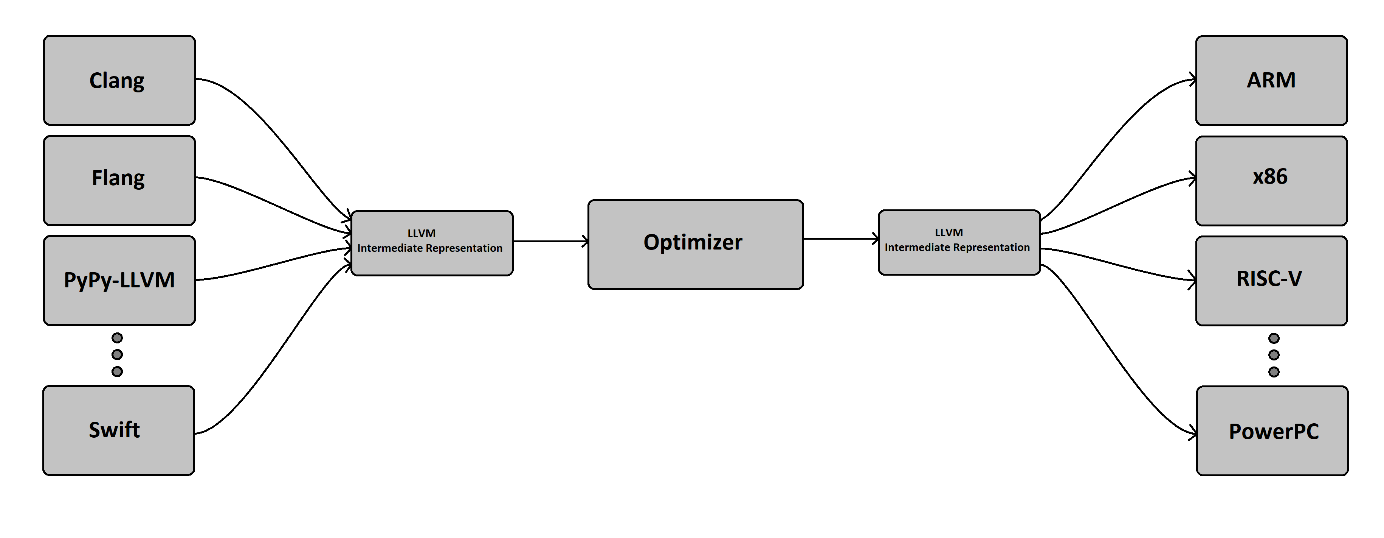
\includegraphics[width=0.8\linewidth]{llvm_diagram.png}
	   \caption{LLVM Frontend ve Backend}
	\end{figure}
\end{frame}

\subsection{LLVM Derleyicisi Backend}
\begin{frame}{Backend}
    \begin{itemize}
        \item Talimat Seçimi (Instruction Selection)
        \item Zamanlama ve Oluşturma
        \item SSA tabanlı Makine Kodu Optimizasyonları
        \item Yazmaç Atama (Register Allocation)
        \item Prolog/Epilog Kodu Ekleme
        \item Kod Yayımı
        \item Bağlama (Linking)
        
    \end{itemize}
\end{frame}

\begin{frame}{Talimat Seçimi Çerçeveleri}
    \begin{itemize}
        \item FastISel
        \item SelectionDAG
        \item GlobalISel
    \end{itemize}
\end{frame}

\begin{frame}{SelectionDAG}
    \begin{enumerate}
    \item 
    İlk DAG'ı Oluştur
    \item
    SelectionDAG'ı Optimize Et
    \item
    SelectionDAG Türlerini Yasallaştır (Legalize Types)
    \item
    SelectionDAG'ı Optimize Et 
    \item
    SelectionDAG İşlemlerini Yasallaştır (Legalize Ops)
    \item
    SelectionDAG'ı Optimize Et
    \item
    DAG'dan talimatları seç
    \item
    SelectionDAG Zamanlama ve Oluşturma
    \end{enumerate}

	\begin{definition}
		\alert{Yönlü Çevrimsiz Grafik (DAG)}, çevrimi olmayan yönlü bir graf'tır.
	\end{definition}
\end{frame}
